\graphicspath{{img/ch1}}

\section{Introduction}
Lunar pits are unique surface features that stand apart from the more familiar impact craters and volcanic vents. With steep, vertical walls and the potential to provide access to subsurface voids like collapsed lava tubes, tectonic caverns, or impact-induced hollow spaces \cite{lunar-pit-distribution, lunar-pits-entrances-to-caves, new-wagner}, these pits have become a focal point for lunar exploration. Their discovery, driven by high-resolution imagery from the Lunar Reconnaissance Orbiter (LRO) Narrow Angle Camera (NAC) and SELENE datasets, has reshaped our understanding of the Moon's crust \cite{lunar-pit-distribution, new-wagner, Carrer2024}. More than geological curiosities, lunar pits are now seen as potential shelters, resource storage sites, and future operational bases \cite{bases-feng, newer-thermal, sublunear-lava}.

Lunar pits offer direct glimpses into the Moon’s hidden layers, challenging existing models of lunar geology. They expose stratigraphic layers, provide evidence of volcanic processes, and reveal subsurface structures \cite{sublunear-lava, lunar-pit-distribution}. This makes them essential to unraveling the Moon’s geological history and better understanding its surface evolution \cite{new-wagner, thermal-lunar-pits, lunar-pits-entrances-to-caves}. As a result, lunar pits are now a key research focus spanning geology, planetary science, and space engineering. Their potential for supporting human exploration also sparks interest in astrobiology, as these subsurface environments might one day support human activity or life-sustaining habitats \cite{bases-feng, newer-thermal, thermal-lunar-pits}.


\begin{figure}[h!]
    \centering
    \begin{subfigure}[c]{0.59\linewidth}
        \centering
        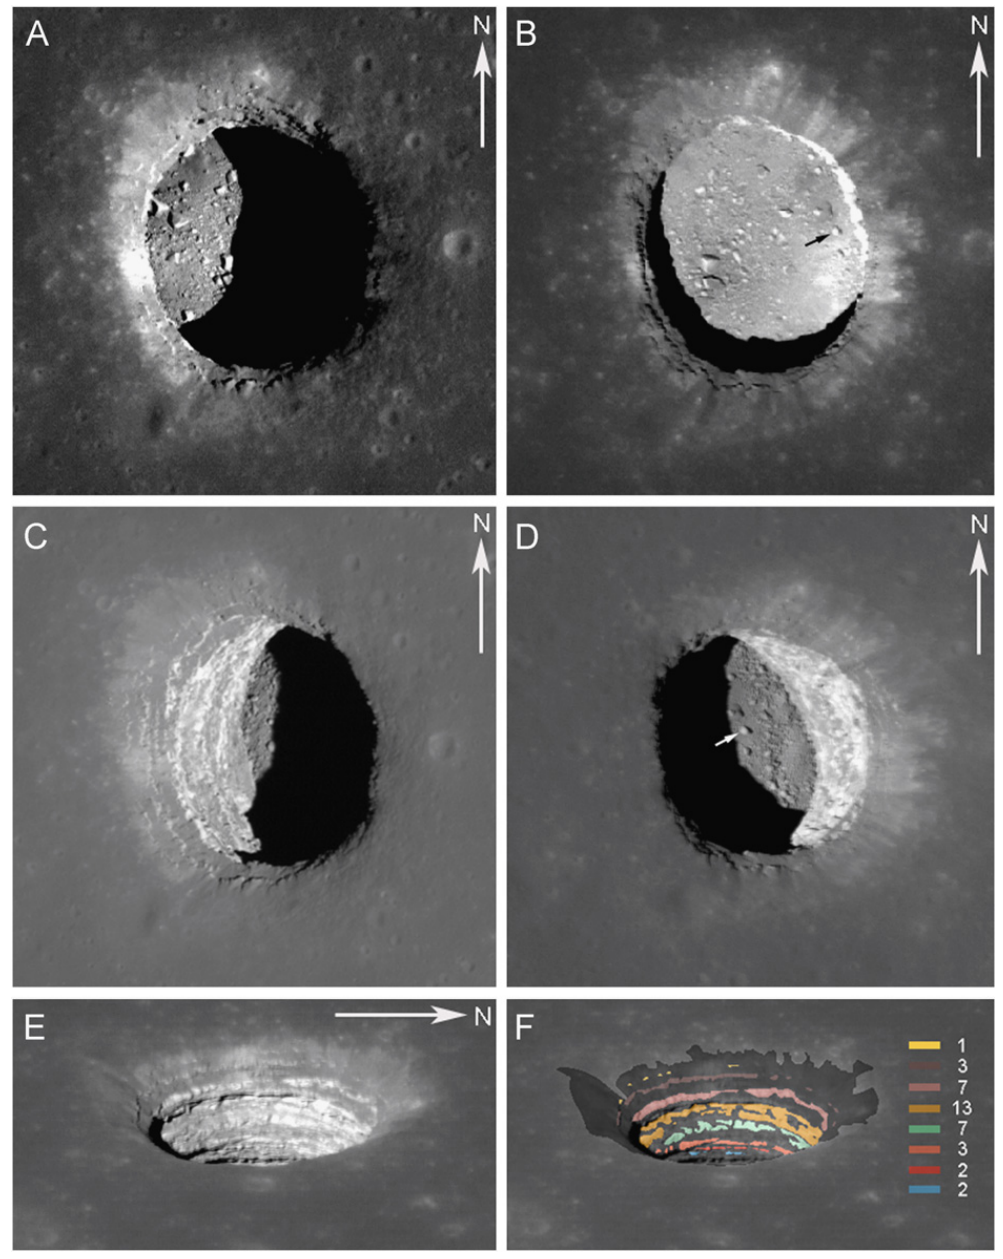
\includegraphics[width=0.9\linewidth]{lunar-pits-with-layers.png}
        \caption{Mare Tranquillitatis lunar pit close-up images from several angles with visible stratigraphic layers (layer segmentation in the figure \textbf{F}). Image A and B reveal more than 90 percent of the lunar pit floor captured with \textbf{LRO NAC}, figure adapted from \cite{sublunear-lava}. }
        \label{fig:image1}
    \end{subfigure}
    \hfill
    \begin{subfigure}[c]{0.4\linewidth}
        \centering
        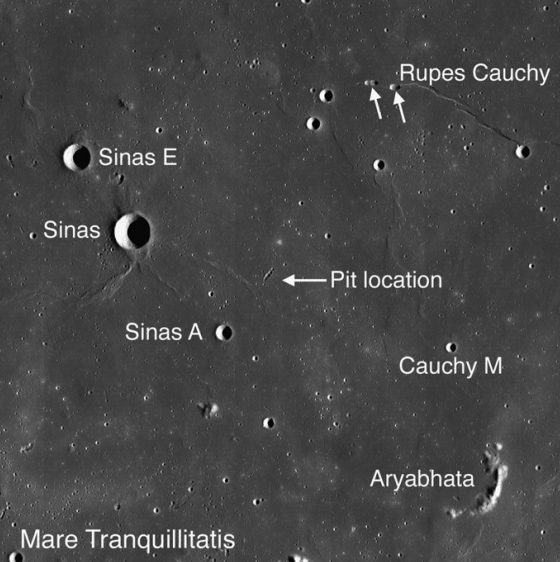
\includegraphics[width=0.9\linewidth]{Lunar_Pit_layers_2pic_location.png}
        \caption{Image of the Mare Tranquillitatis lunar pit location, captured by \textbf{LRO WAC}, figure adapted from \cite{sublunear-lava}}
        \label{fig:image2}
    \end{subfigure}
\end{figure}



\subsection{Discovery and Recognition}
For much of human history, lunar pits remained undiscovered due to their small size and the limitations of early observational technology. Unlike the large and prominent impact craters, pits are small and difficult to detect from Earth-based telescopic observations. It was not until the advent of modern space missions, such as SELENE and LRO, that these features were identified \cite{lunar-pit-distribution}. The high-resolution images captured by the LRO’s Narrow Angle Camera (NAC) revealed steep-walled pits, providing clear evidence of layered and hollow subsurface structures \cite{sublunear-lava, new-wagner, lunar-pit-distribution}.

The realization that lunar pits might grant access to subsurface voids sparked significant interest. Initial discoveries, like the Mare Tranquillitatis pit, shifted these features from mere curiosities to practical exploration targets. Recent radar analysis by Carrer et al. (2024) provided compelling evidence of an accessible cave conduit beneath this pit \cite{Carrer2024}, opening the door to future exploration missions that could access subsurface voids where stable environmental conditions might support human activities \cite{newer-thermal, thermal-lunar-pits, sublunear-lava}.

The significance of lunar pits has grown as radar imaging, 3D modeling, and thermal analysis have advanced \cite{Carrer2024, new-wagner, lunar-pit-distribution}. From early Apollo-era conjectures to present-day confirmations, pits have become essential targets for exploration.
